\documentclass[twoside, 12pt]{article}

\usepackage[sc]{mathpazo} % Use the Palatino font
\usepackage[T1]{fontenc} % Use 8-bit encoding that has 256 glyphs
\linespread{1.5} % Line spacing - Palatino needs more space between lines

%\usepackage[twoside,width=16cm,height=24cm,left=3cm]{geometry}
\usepackage[hmarginratio=1:1,top=20mm,width=20cm,height=23.7cm,columnsep=15pt]{geometry} % Document margins
\usepackage{multicol} % Used for the two-column layout of the document
\usepackage[hang, small,labelfont=bf,up,textfont=it,up]{caption} % Custom captions under/above floats in tables or figures
\usepackage{booktabs} % Horizontal rules in tables
\usepackage{float} % Required for tables and figures in the multi-column environment - they need to be placed in specific locations with the [H] (e.g. \begin{table}[H])
\usepackage{hyperref} % For hyperlinks in the PDF

%----------- Agregados para el caso de ustedes -------------------------------
\usepackage[spanish]{babel}% idioma castellano
\usepackage[utf8]{inputenc}% esto es para poder poner los tildes directamente. Puede que cambie de versión a versión de sistema operativos (más información en http://www.aq.upm.es/Departamentos/Fisica/agmartin/webpublico/latex/FAQ-CervanTeX/FAQ-CervanTeX-6.html )
\usepackage{graphicx} % para insertar figuras
\usepackage{subfigure} % para insertar figuras dentro de figuras
\usepackage{times} % plataforma
\usepackage{amsmath} % --para ecuaciones y algunos símbolos 
\usepackage{wrapfig,lipsum}
% ---------------------- -----------------------------------------------------

\usepackage{lettrine} % The lettrine is the first enlarged letter at the beginning of the text
\usepackage{paralist} % Used for the compactitem environment which makes bullet points with less space between them
\usepackage[T1]{fontenc}					%para poder usar tildes sin problemas

\usepackage{mathrsfs}
% Abreviaturas
\newcommand\RR{\mathbb{R}}

\begin{document}

\begin{center}
{\fontsize{20pt}{10pt}\textbf{Implementación de potenciales y compiladores}}
\end{center}

El objetivo fue generar un método para implementar el cálculo de las fuerzas totales en un sistema de $N_{part}$ partículas para un potencial dado. Esta función \texttt{forces} debía ser tan general como fuese posible para así evitar problemas a la hora de cambiar el potencial.

Estas funciones fueron implementadas en C y, posteriormente, se comparó su velocidad de ejecución para distintas optimizaciones del compilador: \texttt{O0}, \texttt{O1}, \texttt{O2}, \texttt{O3} y \texttt{Ofast}

\section{Implementaciones}
Con esto en mente, se plantearon 9 posibles implementaciones de la función \texttt{forces} combinando distintos rasgos. En todos los casos (excepto el primero), \texttt{forces} llamaba otras funciones para ejecutar el cálculo de la fuerza (\texttt{pair\_force}) o energía (\texttt{pair\_energ}) de interacción entre 2 partículas. 

Los rasgos que se fueron modificando son: 

\begin{quote}
\begin{description}
\item[Precalculo:] El pre-calculo o no de parámetros relevantes para la interacción tanto en la energía como en la fuerza de 2 partículas

\item[Auxiliares:] Separar el cálculo auxiliar en 2 funciones distintas \texttt{pair\_force} y \texttt{pair\_energ} o tener una única función \texttt{pair\_energ\_force}

\item[Modulo:] Que la función auxiliar que calcula la fuerza de interacción devuelva el vector completo (con sus 3 componentes) o solo el módulo.
\end{description}
\end{quote}

Todas estas funciones se compararon con una función \texttt{forces1} sin funciones auxiliares que, en principio, sería la más veloz. Así, fue posible evaluar que tanta velocidad de ejecución se perdía en pos de la encapsulación del potencial. 

\subsection{Estabilización del tiempo de ejecución}

Preliminarmente, se buscó el valor de $N_{part}$ a partir del cual el tiempo de ejecución $\tau$ resultaba \[\tau\sim N^2\] dado que la cantidad de interacciones que \texttt{forces} calculaba es $N(N-1)/2\sim N^2$, bajo la hipótesis de que el tiempo de cómputo de la interacción entre 2 partículas es independiente de sus posiciones. Para asegurar esto último, se evitó la aplicación de un radio de corte.

Esto se hizo calculando el tiempo que tomaba computar $N_{iter}$ veces las fuerzas de un sistema de $N_{part}$ partículas. Los resultados se muestran en la \textbf{Figura \ref{fig:TvsNpart}}

\begin{figure}[h]
	\centering
	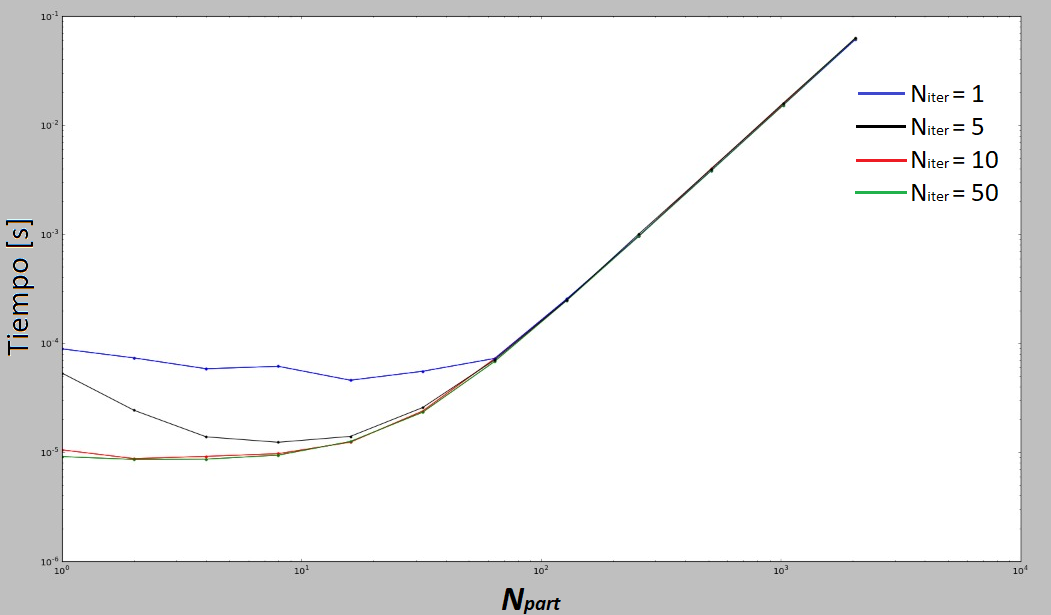
\includegraphics[scale=0.6]{Imagenes/Estabilizacion_Npart.png}
	\caption{Tiempo de ejecución de $N_{iter}$ \texttt{forces} para $N_{part}$ partículas. Para $N_{iter}>10$, el comportamiento se independiza de $N_{iter}$ y para $N_{part}>100$ el tiempo ya es polinómico (cuadrático) para todo $N_{part}$.}
	\label{fig:TvsNpart}
\end{figure}

\subsection{Comparación: Potencial de Morse}

El primer potencial en implementarse fue el potencial (central) de Morse

\[ V_{M} (r) = D\big[1-e^{-\alpha (r-r_{eq})}\big]^2\]

Compilando con los distintos optimizadores \texttt{O} se corrieron las simulaciones para sistemas con $N_{part}=???$. Los tiempos se obtuvieron mediante estadística sobre 100 corridas y se pueden apreciar en la \textbf{Figura \ref{fig:CompTodas}}

\begin{figure}[h]
	\centering
%	\includegraphics[scale=0.6]{}
	\caption{Comparación de tiempos para las distintas implementaciones vía}
	\label{fig:CompTodas}
\end{figure}

ALGO DE ANALISIS

Se destacan las funciones 1, 5 y 9 por su mayor portabilidad, permitiendo usar las 2 funciones auxiliares como \textit{test} directamente desde \texttt{Python} y devolviendo el módulo de fuerza, dado que el vector dirección de la fuerza es independiente del potencial.

\begin{quote}
\begin{description}
\item[1] Sin funciones auxiliares.
\item[5] Dos funciones, con parámetros precalculados, devuelve modulo de fuerza.
\item[9] Dos funciones, sin parámetros precalculados, devuelve modulo de fuerza (encapsula totalmente el potencial).
\end{description}
\end{quote}

Las demás funciones son:

\begin{quote}
\begin{description}
\item[2 y 3] Única función auxiliar \texttt{pair\_energ\_force} con y sin parámetros precalculados.
\item[4] Como \texttt{forces5} pero devolviendo el vector completo
\item[6] Como \texttt{forces9} pero con algunos parámetros precalculados (no todos).
\item[7 y 8] Versiones de \texttt{forces6} y \texttt{forces9} con una única función auxiliar \texttt{pair\_energ\_force}.
\end{description}
\end{quote}

En el caso de \texttt{forces9} es importante aclarar que, al no tener ningún parámetro precalculado, la encapsulación del potencial era completa. Desde el punto de vista de la ingeniería de software \texttt{forces9} sería la óptima. Por lo tanto, se aislaron las funciones \texttt{forces1}, \texttt{forces2} y \texttt{forces3} para cuantificar la pérdida de velocidad en pos de la portabilidad (encapsulación del potencial).

\subsection{Comparación: Potencial de Lennard-Jonnes}

	
\end{document}
